\section{Τίτλος}

\begin{figure}[h!]
    \centering
    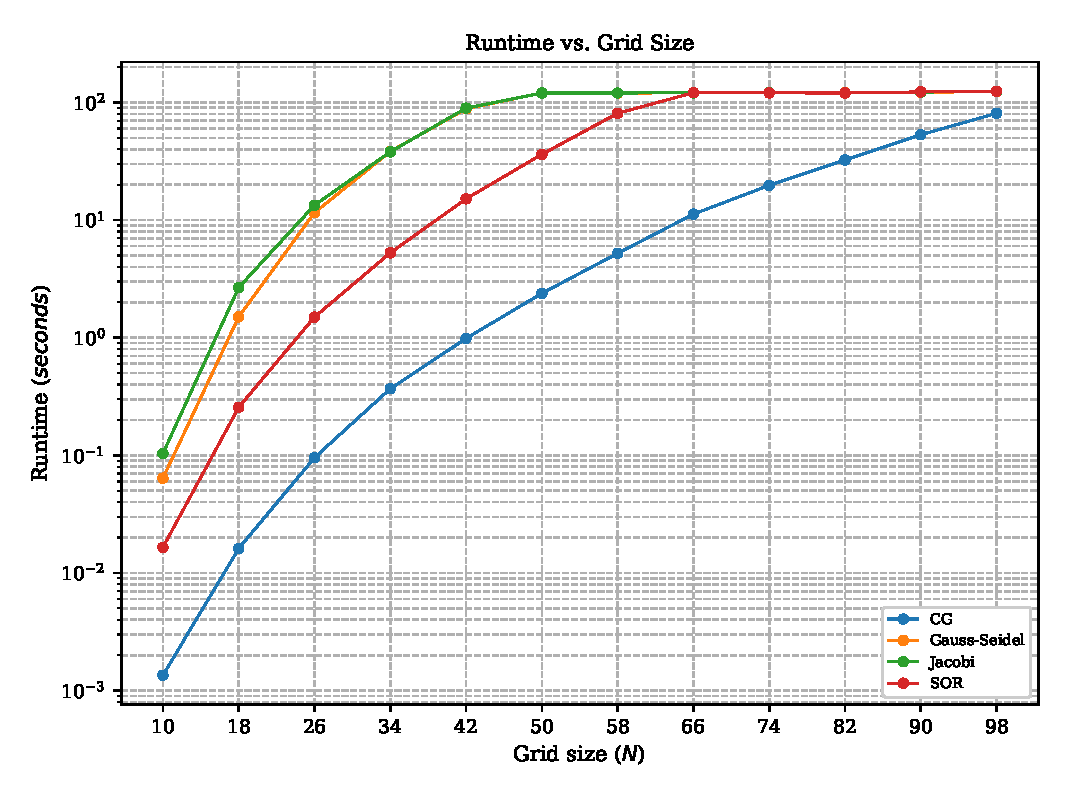
\includegraphics[width=0.80\linewidth]{doc/figures/runtime_gridsize.eps}
    \caption{Σύντομη περιγραφή}
    \label{fig:placeholder}
\end{figure}

\begin{image}
    \centering
    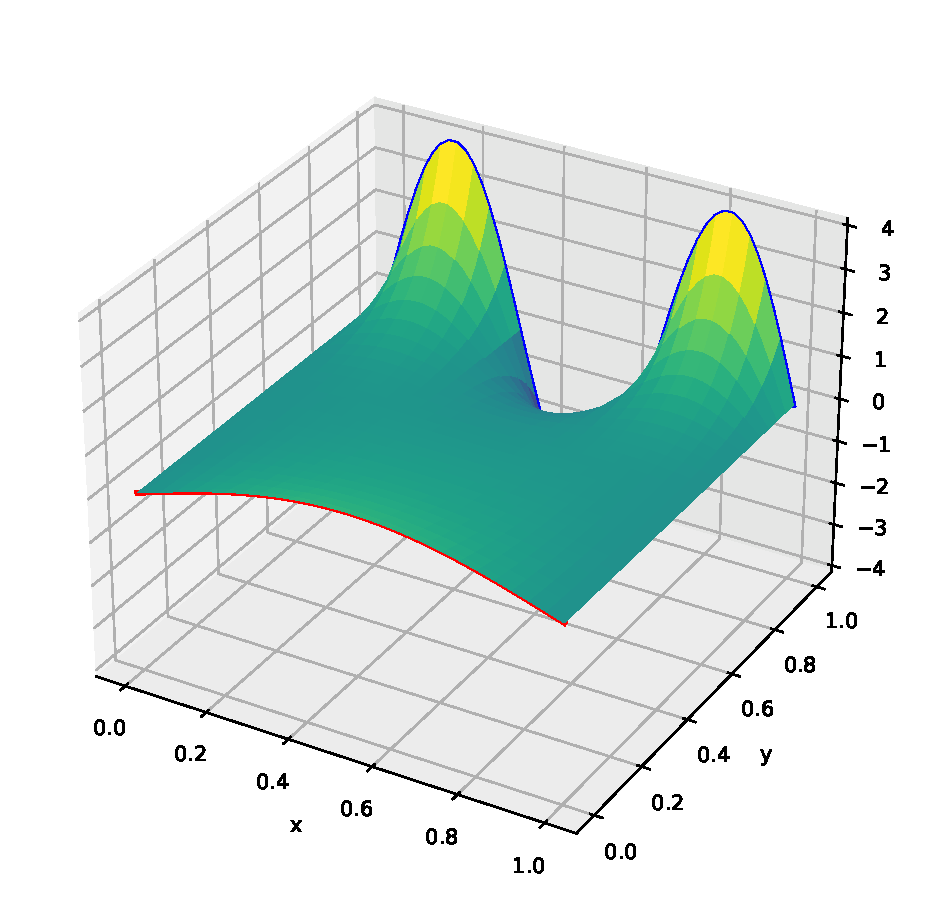
\includegraphics[width=0.70\textwidth]{doc/images/surface_plot.eps}
    \caption{Σύντομη περιγραφή}
    \label{img:example}
\end{image}


\begin{table}[h!]
    \centering
    \begin{tabular}{|c|c|c|c|c|}
    \hline
     N & \en{CG} & \en{Gauss-Seidel} & \en{Jacobi} & \en{SOR} \\
    \hline
    10 & 0.00104029 & 0.068981 & 0.107458 & 0.0152744 \\ \hline
    98 & 87.2408   & 2778.52  & 2843.33  & 1465.69    \\ 
    \hline
    \end{tabular}
    \caption{Σύντομη περιγραφή}
    \label{tab:computation-times}
\end{table}